\documentclass[runningheads]{llncs}

\usepackage[T1]{fontenc}
\usepackage{graphicx}
\usepackage{booktabs}
\usepackage{enumitem}
\usepackage{subcaption}
\usepackage{float}
\usepackage{multirow}
\usepackage{amsmath}
\usepackage{amssymb}
\usepackage{tikz}
\usetikzlibrary{positioning,arrows.meta,shapes.geometric,fit,backgrounds,calc}
\usepackage{xcolor}
\usepackage{microtype}
\usepackage{setspace}
\usepackage[hidelinks]{hyperref}
\renewcommand\UrlFont{\color{blue}\rmfamily}
\urlstyle{rm}
\setlength{\textfloatsep}{5pt plus 1pt minus 2pt}
\setlength{\floatsep}{5pt plus 1pt minus 2pt}
\setlength{\intextsep}{5pt plus 1pt minus 2pt}
\setlength{\abovecaptionskip}{2pt}
\setlength{\belowcaptionskip}{0pt}

\graphicspath{{figures/}}

\newcommand{\macroF}{\textsc{Macro-F1}}

\begin{document}
\setstretch{0.94}

\title{Unifying Heterogeneous IoMT Datasets for Intrusion Detection: From Laboratory Testbeds to Real Hospital Network Evaluation}

\titlerunning{Unifying IoMT Datasets for Intrusion Detection}

\author{Pantelis Petrakis\orcidID{0009-0008-0339-4590} \and Jordi Dom\'{e}nech\orcidID{0000-0002-2977-7265} \and Olga Le\'{o}n\orcidID{0000-0003-2869-051X} \and Isabel V. Martin-Faus\orcidID{0000-0001-9975-8791} \and Josep Pegueroles\orcidID{0000-0002-5194-4883}}

\authorrunning{P. Petrakis et al.}

\institute{Universitat Polit\`{e}cnica de Catalunya (UPC) -- BarcelonaTech, Barcelona 08034, Spain\\
\email{pantelis.petrakis@estudiantat.upc.edu}\\
\email{\{jordi.domenech.fons, olga.leon, isabel.martin-faus, josep.pegueroles\}@upc.edu}}

\maketitle

\begin{abstract}
The growing adoption of Internet of Medical Things (IoMT) devices in healthcare has introduced significant cybersecurity challenges. While machine-learning-based Intrusion Detection Systems (IDS) show promising performance, their practical deployment is hindered by reliance on isolated, single-domain datasets that fail to capture the heterogeneity of the IoMT threat landscape. This paper addresses this critical limitation by proposing a systematic methodology to unify heterogeneous IoMT network traffic datasets into a standardized, ML-ready representation. Using MIOTTA-NPT, a network preprocessing tool that operates directly on raw packet captures, we extract a uniform set of statistical features that resolves feature heterogeneity at the source. We integrate two distinct public datasets (CICIoMT2024 and IoMT-TrafficData) into a unified collection of more than $8 \times 10^{6}$ records and train three tree-based classifiers (Decision Tree, Random Forest, XGBoost) on isolated and unified regimes. Extensive evaluation shows that single-source models collapse under true cross-domain transfer (e.g., B2$\to$CIC \macroF{} $=0.0523$ for DT), whereas models trained on the unified dataset reach \macroF{} up to $0.952$ across both constituent domains. We additionally test the unified models on \textsc{HospNet26}, the first public dataset of real hospital network traffic, comprising $1.26 \times 10^{6}$ unlabelled clinical traffic windows. This real-world evaluation reveals a substantial laboratory-to-clinic covariate shift: $90\%\!-\!96\%$ of benign clinical traffic is misclassified as attack, primarily as DoS. Our results provide the first quantitative measurement of this gap and motivate concrete recalibration strategies for safe deployment of IDS in operational hospital environments.

\keywords{Internet of Medical Things \and Intrusion Detection Systems \and Dataset Unification \and Cross-Domain Generalization \and Real-World Evaluation \and Covariate Shift \and Machine Learning.}
\end{abstract}

\section{Introduction}
\label{sec:intro}

The rapid proliferation of connected medical devices, wearable sensors, and clinical infrastructure has established the Internet of Medical Things (IoMT) as a foundation of modern healthcare delivery~\cite{dimitrov2016medical}. However, this broad connectivity introduces a significantly enlarged attack surface, exposing life-critical devices to severe cyber threats. Unlike traditional IT systems, compromised IoMT devices---such as smart infusion pumps, vital sign monitors, or surgical robots---can directly endanger patient safety~\cite{domenech2024ensuring}. The European Union Agency for Cybersecurity reports a sharp rise in cyberattacks targeting the health sector between 2021 and 2023, with ransomware, data exfiltration and denial-of-service among the most prevalent threat categories~\cite{enisa2023health}. Effective Intrusion Detection Systems (IDS) tailored to the operational constraints of IoMT environments are therefore an urgent need~\cite{domenech2024ensuring}.

Machine-learning-based IDS have emerged as a promising solution that can identify both known and novel attacks by learning behavioural patterns from network traffic~\cite{ahmad2021network}. Their effectiveness, however, depends heavily on the quality, diversity and representativeness of their training data~\cite{khraisat2019survey,Domenech2026}. A critical limitation of current IoMT security research is the reliance on isolated, single-domain datasets that capture only a narrow slice of the attack landscape. Models trained on these independent datasets tend to overfit to specific network topologies and traffic distributions, failing to generalize when deployed in different environments~\cite{domenech2025evaluating,heidari2023iot}.

This dataset isolation problem is compounded by the structural challenge of \emph{feature heterogeneity}. Existing benchmark datasets employ structurally incompatible feature extraction methodologies. CICIoMT2024~\cite{dadkhah2024ciciomt} produces flow-based features extracted with the CICFlowMeter framework~\cite{cicflowmeter}, while IoMT-TrafficData~\cite{areia2024iomt} relies on Zeek-derived per-connection records~\cite{zeek}. Because these tools yield semantically and structurally different feature spaces, direct dataset integration or cross-domain learning is inherently impossible without returning to the raw packet captures (PCAPs).

A second, even more profound gap exists in the current literature regarding \emph{operational} deployment of these systems: to the best of our knowledge, no machine-learning-based IDS for IoMT has been rigorously evaluated against \emph{real} clinical traffic captured from a live hospital network. Existing evaluations are restricted to laboratory testbeds or synthetic datasets, leaving the models' generalizability to live hospital networks entirely unproven~\cite{domenech2024ensuring,sommer2010outside}. Real medical networks involve complex, high-throughput traffic mixtures (medical imaging streams, electronic health records, proprietary clinical protocols, administrative systems) that introduce a ``laboratory-to-clinic'' covariate shift not captured by synthetic data. Without confronting this distributional shift, the operational readiness of these models remains unknown.

This paper addresses both barriers by systematically unifying heterogeneous IoMT datasets and rigorously evaluating model generalizability on both laboratory testbeds and a real-world clinical network. Our main contributions are:

\begin{enumerate}[nosep,leftmargin=*]
  \item \textbf{Systematic PCAP-level dataset unification via MIOTTA-NPT.} We propose a comprehensive methodology that resolves feature heterogeneity at the source. Using MIOTTA-NPT~\cite{leon2025miotta,miotta_npt_github}, a network preprocessing tool that operates directly on raw PCAP files, we extract an identical statistical feature representation from two heterogeneous public IoMT datasets (CICIoMT2024 and IoMT-TrafficData). Combined with a three-level label harmonization scheme and rigorous data quality assurance, our pipeline integrates these sources into a cohesive, ML-ready dataset of more than $8 \times 10^{6}$ records.

  \item \textbf{Quantification of single-source collapse versus unified generalizability.} We evaluate Decision Tree, Random Forest and XGBoost classifiers under three regimes (CIC-only, IoMT-only, Unified). Single-source models fail under cross-domain transfer (opposite-source \macroF{} drops to $0.0523$--$0.3423$, depending on regime/model), whereas unified models achieve \macroF{} $\geq 0.926$ on both source-specific test slices simultaneously, with the best model reaching $0.952$ on the full mixed test set. We complement these results with paired McNemar's tests to confirm statistical and practical significance.

  \item \textbf{First real-world evaluation on \textsc{HospNet26}.} We deploy the unified models on \textsc{HospNet26}~\cite{hospnet26,Domenech2026_cbms}, a recently released dataset of $1.26 \times 10^{6}$ unlabelled traffic windows from a live German hospital network. The evaluation reveals a significant covariate shift: only $3.7\%\!-\!10.0\%$ of clinical traffic is classified as benign, with most predictions concentrated in DoS-like classes. To the best of our knowledge, this is the first quantitative measurement of the laboratory-to-clinic gap for IoMT IDS. We complement this finding with concrete recalibration strategies (few-shot benign fine-tuning and post-hoc threshold calibration) that provide actionable guidance for closing the gap.
\end{enumerate}

The remainder of the paper is organised as follows. Section~\ref{sec:background} reviews related work on IoMT security, ML-based IDS and dataset integration. Section~\ref{sec:methodology} details the proposed unification methodology. Section~\ref{sec:setup} presents the experimental setup. Section~\ref{sec:results_1} reports the cross-domain evaluation on the public datasets. Section~\ref{sec:results_2} presents the real-world evaluation on \textsc{HospNet26}. Section~\ref{sec:discussion} discusses implications and recalibration strategies. Section~\ref{sec:conclusion} concludes the paper.

\section{Background and Related Work}
\label{sec:background}

\subsection{IoMT Security and ML-Based IDS}

The IoMT ecosystem comprises networked medical instruments operating over heterogeneous protocols (Wi-Fi, Bluetooth Low Energy, MQTT, CoAP, Zigbee), often with limited computational resources and long deployment lifetimes~\cite{dimitrov2016medical}. Traditional signature-based IDS struggle in this environment because attack patterns evolve faster than rule databases can be updated, and proprietary medical protocols are seldom modelled by generic detection rules~\cite{khraisat2019survey}.

Machine-learning-based IDS---in particular tree ensembles, deep learning models and hybrid pipelines---have been proposed to overcome these limitations~\cite{ahmad2021network,heidari2023iot}. Hady et al.~\cite{hady2020ids} compared shallow and deep models on combined medical and network data, while Hussain et al.~\cite{hussain2021framework} proposed a malicious-traffic detection framework targeting healthcare IoT. Maim\'{o} et al.~\cite{maimo2019intelligent} addressed ransomware mitigation in integrated clinical environments. A recent systematic review~\cite{domenech2024ensuring} surveys behaviour-based IDS approaches for IoMT, identifying lack of dataset diversity and absence of real clinical evaluations as principal open problems.

\subsection{Datasets for IoMT and IoT Intrusion Detection}

The community has produced several benchmark datasets, but each captures only a subset of the threat landscape and uses incompatible feature representations. \textbf{CICIoMT2024}~\cite{dadkhah2024ciciomt} is a multi-protocol IoMT dataset with $18$ attack types extracted via the CICFlowMeter framework and supplied as flow-based CSV records. \textbf{IoMT-TrafficData}~\cite{areia2024iomt} provides hospital-oriented testbed traffic with Zeek-derived per-connection statistics. \textbf{CICIoT2023}~\cite{neto2023ciciot2023} is a large-scale general-purpose IoT dataset, while several other datasets exist for general IoT (e.g.\ Bot-IoT, TON-IoT, IoT-23). All were developed independently, with different network topologies, device populations, and---crucially---different feature extraction tools. Direct concatenation across datasets is therefore not possible.

More recently, an additional line of research has shifted from laboratory traces to \emph{real} clinical network traffic. \textbf{HospNet26}~\cite{hospnet26,Domenech2026_cbms} provides anonymized statistical features from one week of real internal traffic from a Helios hospital in Germany. It is supplied in three feature granularities (flow, window, combined) and contains no attack labels: it is a pure benign-traffic reference for evaluating specificity in operational environments. To date, no published work has used \textsc{HospNet26} to evaluate the deployment behaviour of cross-dataset-trained IDS models.

\subsection{Dataset Unification Approaches}

Unifying heterogeneous datasets has been investigated for general NIDS benchmarking. Khan et al.~\cite{khan2024umnids} propose META, a multi-modal unified dataset for NIDS, and Noblet et al.~\cite{noblet2025nxcap} propose Nxcap as a unified benchmark format. Federated approaches~\cite{abouhouran2025federated} address dataset isolation without explicit data centralisation. None of these works addresses the IoMT-specific combination of heterogeneous tooling, real clinical data, and cross-domain evaluation that we tackle in this study.

The MIOTTA research group has previously released MIOTTA-NPT~\cite{leon2025miotta,miotta_npt_github}, a configurable preprocessing tool that converts raw PCAPs into both per-window statistical features (similar in spirit to CICFlowMeter or Zeek) and per-packet binary representations inspired by nPrint~\cite{holland2021nprint}. The tool's window-based mode produces a uniform feature space across arbitrary input PCAPs, which is the key enabler for the dataset integration pipeline described in the next section.

\subsection{Gap Analysis}

Three gaps motivate this work. First, no prior study has \emph{integrated} CICIoMT2024 and IoMT-TrafficData at the raw-PCAP level, despite both being widely cited IoMT IDS benchmarks with non-overlapping attack coverage. Second, no prior IoMT IDS has been evaluated on \textsc{HospNet26}, leaving the laboratory-to-clinic gap uncharacterised. Third, prior cross-domain studies in IoMT/IoT IDS rely on heuristic feature alignment or direct CSV concatenation, both of which preserve tool-induced biases. Our contribution closes all three gaps simultaneously.

\section{Proposed Unification Methodology}
\label{sec:methodology}

\subsection{Pipeline Overview}

The proposed pipeline applies five stages to each source dataset (Fig.~\ref{fig:pipeline}): (i) PCAP collection; (ii) feature extraction via MIOTTA-NPT; (iii) three-level label harmonization; (iv) quality assurance; (v) cross-source merging with provenance attribution and stratified splitting, yielding a single ML-ready Parquet/CSV dataset for training and cross-domain evaluation. The unified dataset can be found in \cite{pantelis2026_unified_dataset}.

Across both sources, CICIoMT2024 provides $18$ attack sub-types (DDoS, DoS, MQTT, Spoofing, Reconnaissance variants) and IoMT-TrafficData adds $8$ further sub-types (DoS, MQTT, Reconnaissance, Spoofing; no DDoS), yielding $26$ fine-grained labels in total---all mapped to six shared categorical classes by stage~(iii).

\begin{figure}[H]
\vspace*{-1.5mm}
\centering
\scalebox{0.84}{%
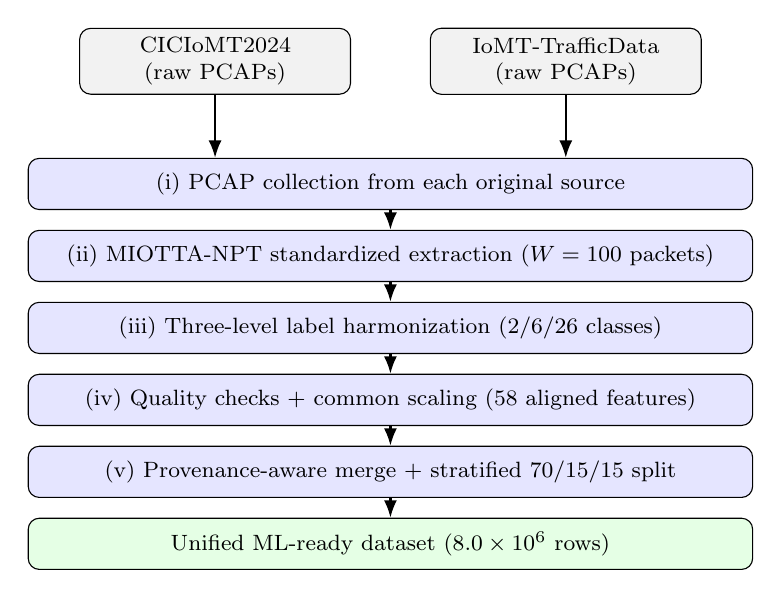
\begin{tikzpicture}[
  node distance=2.5mm and 10mm,
  srcnode/.style={rectangle, draw, rounded corners, minimum width=34mm, minimum height=7mm, text width=32mm, align=center, fill=gray!10, font=\footnotesize, inner sep=1.2mm},
  stage/.style={rectangle, draw, rounded corners, minimum width=92mm, minimum height=6.5mm, align=left, fill=blue!10, font=\footnotesize, inner sep=1.6mm},
  outnode/.style={rectangle, draw, rounded corners, minimum width=92mm, minimum height=6.5mm, align=left, fill=green!10, font=\footnotesize, inner sep=1.6mm},
  arr/.style={-{Latex[length=2.2mm]}, thick}
]
\node (cic) [srcnode] {CICIoMT2024\\(raw PCAPs)};
\node (iomt) [srcnode, right=of cic] {IoMT-TrafficData\\(raw PCAPs)};

\coordinate (srcjoin) at ($(cic.south)!0.5!(iomt.south)$);
\node (s1) [stage, below=8mm of srcjoin] {(i) PCAP collection from each original source};
\node (s2) [stage, below=of s1] {(ii) MIOTTA-NPT standardized extraction ($W=100$ packets)};
\node (s3) [stage, below=of s2] {(iii) Three-level label harmonization (2/6/26 classes)};
\node (s4) [stage, below=of s3] {(iv) Quality checks + common scaling (58 aligned features)};
\node (s5) [stage, below=of s4] {(v) Provenance-aware merge + stratified 70/15/15 split};
\node (final) [outnode, below=of s5] {Unified ML-ready dataset ($8.0\times10^{6}$ rows)};

\draw [arr] (cic.south) -- (cic.south |- s1.north);
\draw [arr] (iomt.south) -- (iomt.south |- s1.north);
\draw [arr] (s1.south) -- (s2.north);
\draw [arr] (s2.south) -- (s3.north);
\draw [arr] (s3.south) -- (s4.north);
\draw [arr] (s4.south) -- (s5.north);
\draw [arr] (s5.south) -- (final.north);
\end{tikzpicture}%
}
\vspace{3pt}
{\setlength{\abovecaptionskip}{7pt}\caption{Five-stage unification pipeline. Heterogeneous IoMT PCAPs from two sources are reduced to a common $58$-feature space by MIOTTA-NPT, harmonized at three label granularities, quality-checked and stratified-split, yielding a single ML-ready dataset with full source provenance.}}
\label{fig:pipeline}
\end{figure}

\subsection{Standardized Feature Extraction via MIOTTA-NPT}

MIOTTA-NPT~\cite{leon2025miotta,miotta_npt_github} is the cornerstone of feature unification. Its \emph{combined} mode operates on raw PCAPs by sliding a fixed-size packet window (here, $W = 100$ packets) over the capture and computing a $73$-dimensional vector of statistical features per window: protocol-level indicators (TCP, UDP, ICMP, MQTT, DNS\dots), TCP flag counts, header lengths and TTLs, window-aggregated packet rates, byte rates, payload sizes, inter-arrival times, statistical moments (mean, standard deviation, covariance, max, min, weighted average) and similar quantities. The output is a uniform tabular representation regardless of the original PCAP source.

Applying MIOTTA-NPT separately to the CICIoMT2024 and IoMT-TrafficData PCAP collections yields two datasets that are \emph{structurally identical} at the feature level: same column names, same data types, same semantics. Direct row-wise concatenation is therefore syntactically valid by construction. Near-zero-variance features (e.g.\ a protocol indicator that is always zero in both sources, owing to absence of that protocol in either testbed) are removed in a final cleaning step, leaving a final feature space of $58$ numeric columns. This eliminates the structural barrier that prevents naive integration of CSV-level features extracted by different tools.

\subsection{Three-Level Label Harmonization}

CICIoMT2024 and IoMT-TrafficData use overlapping but non-identical attack taxonomies. We harmonize them at three granularities:
\begin{itemize}[nosep,leftmargin=*]
  \item \textbf{Binary level:} \texttt{Benign} vs.\ \texttt{Attack}.
  \item \textbf{Categorical level (six classes):} \texttt{Benign}, \texttt{DDoS}, \texttt{DoS}, \texttt{MQTT}, \texttt{Reconnaissance}, \texttt{Spoofing}. This level is the primary classification target throughout the paper. The mapping resolves divergent naming conventions (e.g.\ \texttt{DDoS\_TCP\_Flood} and \texttt{TCP\_DDoS} both map to \texttt{DDoS}) and groups protocol-specific attacks under a unified \texttt{MQTT} category.
  \item \textbf{Fine-grained level:} the original $26$ attack labels are preserved verbatim, enabling future research that requires sub-category specificity.
\end{itemize}

The categorical mapping was designed in collaboration with the IDS literature on IoMT/IoT attack taxonomies~\cite{khraisat2019survey,heidari2023iot} and validated against the original dataset documentation.
In the published merged release, all three target granularities are retained together (\texttt{label\_binary}, \texttt{label\_category}, \texttt{label\_fine}), so downstream studies can directly benchmark 2-class, 6-class, and 26-class settings from the same data asset.

\subsection{Quality Assurance, Scaling and Splitting}

After concatenation, the dataset is subjected to a structural integrity audit that verifies (i) absence of NaN and infinity values across all $58$ numeric features, (ii) type consistency, (iii) per-record presence of all three label columns and four provenance columns (\texttt{source\_dataset}, \texttt{source\_file}, \texttt{attack\_type}, \texttt{attack\_group}). The dataset is split using stratified $70/15/15$ partitioning at the categorical level, preserving class proportions across train/validation/test. The training partition is then used to fit a \texttt{StandardScaler} that is applied to all three partitions, with no refitting on validation/test data to prevent leakage. The same scaler is later reused for the \textsc{HospNet26} evaluation in Section~\ref{sec:results_2}.

\subsection{Provenance Attribution and Cross-Domain Evaluation Design}

Each record retains a \texttt{source\_dataset} field, enabling the construction of three training regimes (CIC-only, IoMT-only, Unified) that all share identical preprocessing, identical splits and identical hyperparameter budgets. The only difference between regimes is which subset of training rows each model sees. This design isolates the effect of dataset integration from confounding factors such as feature engineering or scaler drift, allowing causal attribution of observed performance differences to the data composition.

\section{Experimental Setup}
\label{sec:setup}

\subsection{Unified Dataset Profile}

The integration produces a unified dataset of $8{,}011{,}534$ records across $58$ numeric features \cite{pantelis2026_unified_dataset}. CICIoMT2024 contributes $97.70\%$ of records, IoMT-TrafficData $2.30\%$. The categorical class distribution is shown in Table~\ref{tab:class-balance}: the dataset is heavily attack-dominated ($99.33\%$ attacks vs.\ $0.67\%$ benign), with a $\sim$$575{:}1$ maximum-to-minimum class ratio between DDoS and Spoofing. Train/validation/test partitions contain $5{,}608{,}073$, $1{,}201{,}730$ and $1{,}201{,}731$ records respectively (exactly $70/15/15$).

\begin{table}[H]
\centering
\caption{Categorical class distribution with per-source contribution in the unified dataset.}\label{tab:class-balance}
\small
\resizebox{\textwidth}{!}{%
\begin{tabular}{@{}lrrrr@{}}
\toprule
\textbf{Category} & \textbf{CICIoMT2024} & \textbf{IoMT-TrafficData} & \textbf{Unified records} & \textbf{Unified proportion} \\
\midrule
DDoS           & 5{,}368{,}292 & \phantom{0,000}0 & 5{,}368{,}292 & 67.01\% \\
DoS            & 2{,}100{,}735 & 47{,}742 & 2{,}148{,}477 & 26.82\% \\
MQTT           & \phantom{0,}320{,}204 & 65{,}734 & \phantom{0,}385{,}938 & 4.82\% \\
Benign         & \phantom{0,00}23{,}133 & 30{,}323 & \phantom{0,0}53{,}456 & 0.67\% \\
Reconnaissance & \phantom{0,00}13{,}147 & 32{,}879 & \phantom{0,0}46{,}026 & 0.57\% \\
Spoofing       & \phantom{0,000}1{,}782 & \phantom{0,}7{,}563 & \phantom{0,00}9{,}345 & 0.12\% \\
\midrule
\textbf{Total} & \textbf{7{,}827{,}293} & \textbf{184{,}241} & \textbf{8{,}011{,}534} & \textbf{100\%} \\
\bottomrule
\end{tabular}
}
\end{table}

\subsection{Training Regimes}

To isolate the effect of integration, three regimes are defined:
\begin{itemize}[nosep,leftmargin=*]
  \item \textbf{B1 (CIC-only):} only rows with \texttt{source\_dataset = CICIoMT2024} \cite{dadkhah2024ciciomt}.
  \item \textbf{B2 (IoMT-only):} only rows with \texttt{source\_dataset = IoMT-TrafficData} \cite{areia2024iomt}.
  \item \textbf{U (Unified):} the complete training set (both sources) \cite{pantelis2026_unified_dataset}.
\end{itemize}
Filtering is applied to the existing stratified splits, preserving non-overlapping partition boundaries. All regimes share the same hyperparameter search space, the same iteration budget and the same evaluation protocol.

\subsection{Models and Imbalance Handling}

Three tree-based classifiers of increasing complexity are evaluated: Decision Tree (DT), Random Forest (RF) and XGBoost. Tree-based models have been shown to match or outperform deep learning on tabular data~\cite{grinsztajn2022tree} and natively handle multi-class classification. For DT and RF, we use the same balanced weighting as scikit-learn's \texttt{class\_weight='balanced'}, implemented explicitly as a per-class dictionary passed to \texttt{class\_weight}. For XGBoost (\texttt{multi:softmax}), we pass a \texttt{sample\_weight} vector of length $N_{\mathrm{train}}$: for each training row $i$ with label $y_i=c$, the weight is $w_c = N_{\mathrm{train}}/(K_{\mathrm{train}}\,n_c)$, where $n_c$ is the number of training rows in class $c$ and $K_{\mathrm{train}}$ is the number of \emph{distinct} classes present in that regime's training split (six for B1 and U; five for B2 because DDoS is absent). SMOTE-style oversampling is not used: the dataset already contains $>8 \times 10^{6}$ records, and class weights provide sufficient gradient signal for minority classes.

A globally consistent \texttt{LabelEncoder} (alphabetical order) is used so that confusion matrices remain directly comparable across regimes even when a regime omits a class (B2 lacks DDoS). For B2, XGBoost requires contiguous class IDs, so a thin wrapper temporarily remaps the five present classes to a local range during training and restores the global six-class IDs at prediction time.

\subsection{Hyperparameter Tuning}

\begin{table}[H]
\centering
\caption{Randomized search ($n{=}50$, 3-fold CV, \macroF{}, seed $42$). RF/XGB (B1, U): $300\mathrm{k}$ train subsample, then refit on full train.}\label{tab:hparam-search}
\footnotesize
\setlength{\tabcolsep}{4pt}
\renewcommand{\arraystretch}{1.0}
\begin{tabular}{@{}c l p{0.52\textwidth}@{}}
\toprule
 & \textbf{Hyperparameter} & \textbf{Candidate values} \\
\midrule
\multirow{5}{*}{\textbf{DT}}
& \texttt{max\_depth} & $\{5,10,15,20,25,30,\mathrm{none}\}$ \\
& \texttt{min\_samples\_split} & $\{2,5,10,20,50\}$ \\
& \texttt{min\_samples\_leaf} & $\{1,2,5,10,20\}$ \\
& \texttt{criterion} & $\{\mathrm{gini},\mathrm{entropy}\}$ \\
& \texttt{max\_features} & $\{\sqrt{d},\log_2 d,\mathrm{all}\}$ \\
\midrule
\multirow{7}{*}{\textbf{RF}}
& \texttt{n\_estimators} & $\{100,200,300,500\}$ \\
& \texttt{max\_depth} & $\{10,15,20,25,30,\mathrm{none}\}$ \\
& \texttt{max\_features} & $\{\sqrt{d},\log_2 d,0.3,0.5\}$ \\
& \texttt{min\_samples\_split} & $\{2,5,10,20,50\}$ \\
& \texttt{min\_samples\_leaf} & $\{1,2,5,10,20\}$ \\
& \texttt{max\_samples} & $\{0.5,0.7,0.8,1.0\}$ \\
& \texttt{class\_weight} & $\{\texttt{balanced},\texttt{balanced\_subsample}\}$ \\
\midrule
\multirow{9}{*}{\textbf{XGB}}
& \texttt{learning\_rate} & $\{0.01,0.03,0.05,0.1,0.2,0.3\}$ \\
& \texttt{n\_estimators} & $\{100,200,300,500,1000\}$ \\
& \texttt{max\_depth} & $\{3,5,7,9,12\}$ \\
& \texttt{min\_child\_weight} & $\{1,3,5,10,20\}$ \\
& \texttt{subsample} & $\{0.6,0.7,0.8,0.9,1.0\}$ \\
& \texttt{colsample\_bytree} & $\{0.6,0.7,0.8,0.9,1.0\}$ \\
& \texttt{gamma} & $\{0,0.1,0.5,1,5\}$ \\
& \texttt{reg\_lambda} & $\{0.01,0.1,1,10\}$ \\
& \texttt{reg\_alpha} & $\{0,0.01,0.1,1\}$ \\
\midrule
\multicolumn{3}{@{}p{0.96\linewidth}@{}}{\emph{Fixed:} DT/RF balanced weights (\S\ref{sec:setup}); XGB \texttt{hist}, \texttt{multi:softmax}, \texttt{n\_jobs=1}; CV \texttt{fit} uses \texttt{sample\_weight}.} \\
\bottomrule
\end{tabular}
\renewcommand{\arraystretch}{1}
\end{table}

\subsection{Metrics}

The primary metric is \macroF{}, which weights all six classes equally and is therefore appropriate for imbalanced multi-class evaluation. Weighted-F1 and accuracy are reported as secondary metrics; per-class precision, recall and F1, and normalized confusion matrices, complete the picture. For pairwise comparison of two classifiers on the \emph{same} held-out test set we use McNemar's test~\cite{mcnemar1947note} (Yates correction); Section~\ref{subsec:mcnemar} motivates this choice relative to alternative tests and reports effect sizes alongside $p$-values.

\section{Evaluation on Public Heterogeneous Datasets}
\label{sec:results_1}

\subsection{Cross-Domain Collapse of Single-Source Models}

Table~\ref{tab:cross-domain} reports the \macroF{} of all three classifiers when trained on a single source (B1 or B2) and tested on each of the three test slices (CIC-only, IoMT-only, full mixed). The pattern is unambiguous: in-domain scores are strong (\macroF{} $\geq 0.91$), but on the \emph{opposite} source's slice the scores collapse---to as low as $0.05$ (B2$\to$CIC, DT) and $0.06$ (B2$\to$CIC, RF). XGBoost, despite being the strongest model overall, also collapses to $0.11$ on the same slice. The full-mixed-test scores (which contain both sources in their natural proportion) reflect this collapse: B1 reaches at most $0.74$ and B2 stays below $0.40$.

\begin{table}[H]
\centering
\caption{Tuned single-source models: \macroF{} on the three test slices. Cross-domain entries (the off-source slice) are highlighted by their dramatic drop from the in-domain baseline.}\label{tab:cross-domain}
\small
\begin{tabular}{@{}lcccc@{}}
\toprule
\textbf{Regime} & \textbf{Model} & \textbf{CIC slice} & \textbf{IoMT slice} & \textbf{Full test} \\
\midrule
\multirow{3}{*}{B1 (CIC-only)}  & DT  & 0.9226 (in) & 0.2474 (cross) & 0.6959 \\
                                & RF  & 0.9149 (in) & 0.3423 (cross) & 0.7395 \\
                                & XGB & 0.9410 (in) & 0.2724 (cross) & 0.7199 \\
\midrule
\multirow{3}{*}{B2 (IoMT-only)} & DT  & 0.0523 (cross) & 0.8332 (in) & 0.3284 \\
                                & RF  & 0.0586 (cross) & 0.8333 (in) & 0.2029 \\
                                & XGB & 0.1079 (cross) & 0.8333 (in) & 0.3708 \\
\bottomrule
\end{tabular}
\end{table}

This collapse confirms that single-source models overfit to source-specific traffic statistics. The asymmetric severity (B2$\to$CIC is worse than B1$\to$IoMT) is structurally explained by the absence of DDoS in IoMT-TrafficData: a model trained on B2 has never seen DDoS traffic and therefore cannot recognise the dominant attack class of the CIC test slice.

\subsection{Models Trained on the Unified Dataset Resolve the Cross-Domain Gap}
\label{subsec:unified-resolve}

We now turn to the three classifiers trained under regime U---i.e.\ on the \emph{full unified training split} that mixes both sources---and tested on the same three slices used above. Table~\ref{tab:unified} reports their scores: all three reach \macroF{} $\geq 0.926$ on the CIC slice, $\geq 0.999$ on the IoMT slice (five present classes), and $\geq 0.948$ on the full mixed test. The jump from the best single-source full-test score ($0.7395$, RF-B1) to the weakest unified-trained model ($0.9480$, DT-U) is $+20.85$ pp---far larger than the $0.42$ pp spread among the three unified-trained models---so \emph{training on the unified dataset is the dominant factor} for cross-domain generalisation, well above model choice.

\begin{table}[H]
\centering
\caption{Tuned Unified models: \macroF{} on the three test slices. The IoMT slice value with $^{*}$ is computed over the five present classes (Benign, DoS, MQTT, Reconnaissance, Spoofing); see footnote.}\label{tab:unified}
\small
\begin{tabular}{@{}lccc@{}}
\toprule
\textbf{Model} & \textbf{CIC slice} & \textbf{IoMT slice} & \textbf{Full test} \\
\midrule
Decision Tree & 0.9262 & $0.9990^{*}$ & 0.9480 \\
Random Forest & 0.9285 & $0.9995^{*}$ & 0.9487 \\
XGBoost       & 0.9382 & $0.9999^{*}$ & \textbf{0.9522} \\
\bottomrule
\end{tabular}

\vspace{0.1em}
\raggedright\footnotesize
$^{*}$\,No DDoS in IoMT slice; naive six-class \macroF{} there is $\approx 0.832$. We report five-class \macroF{} for a faithful per-class view; full-test remains the global metric.
\end{table}

\subsection{Per-Class Behaviour of the Best Unified Model}

Fig.~\ref{fig:cm-unified} shows the normalized confusion matrix of the tuned XGBoost-U model on the full test set. Four of the six categories (Benign, MQTT, Reconnaissance, Spoofing) are classified with F1 $\geq 0.98$, even though Spoofing represents only $0.12\%$ of the data---a direct consequence of class-balanced training. Per-class F1 across all three classifiers is summarised in Fig.~\ref{fig:perclass}.

\begin{figure}[H]
\centering
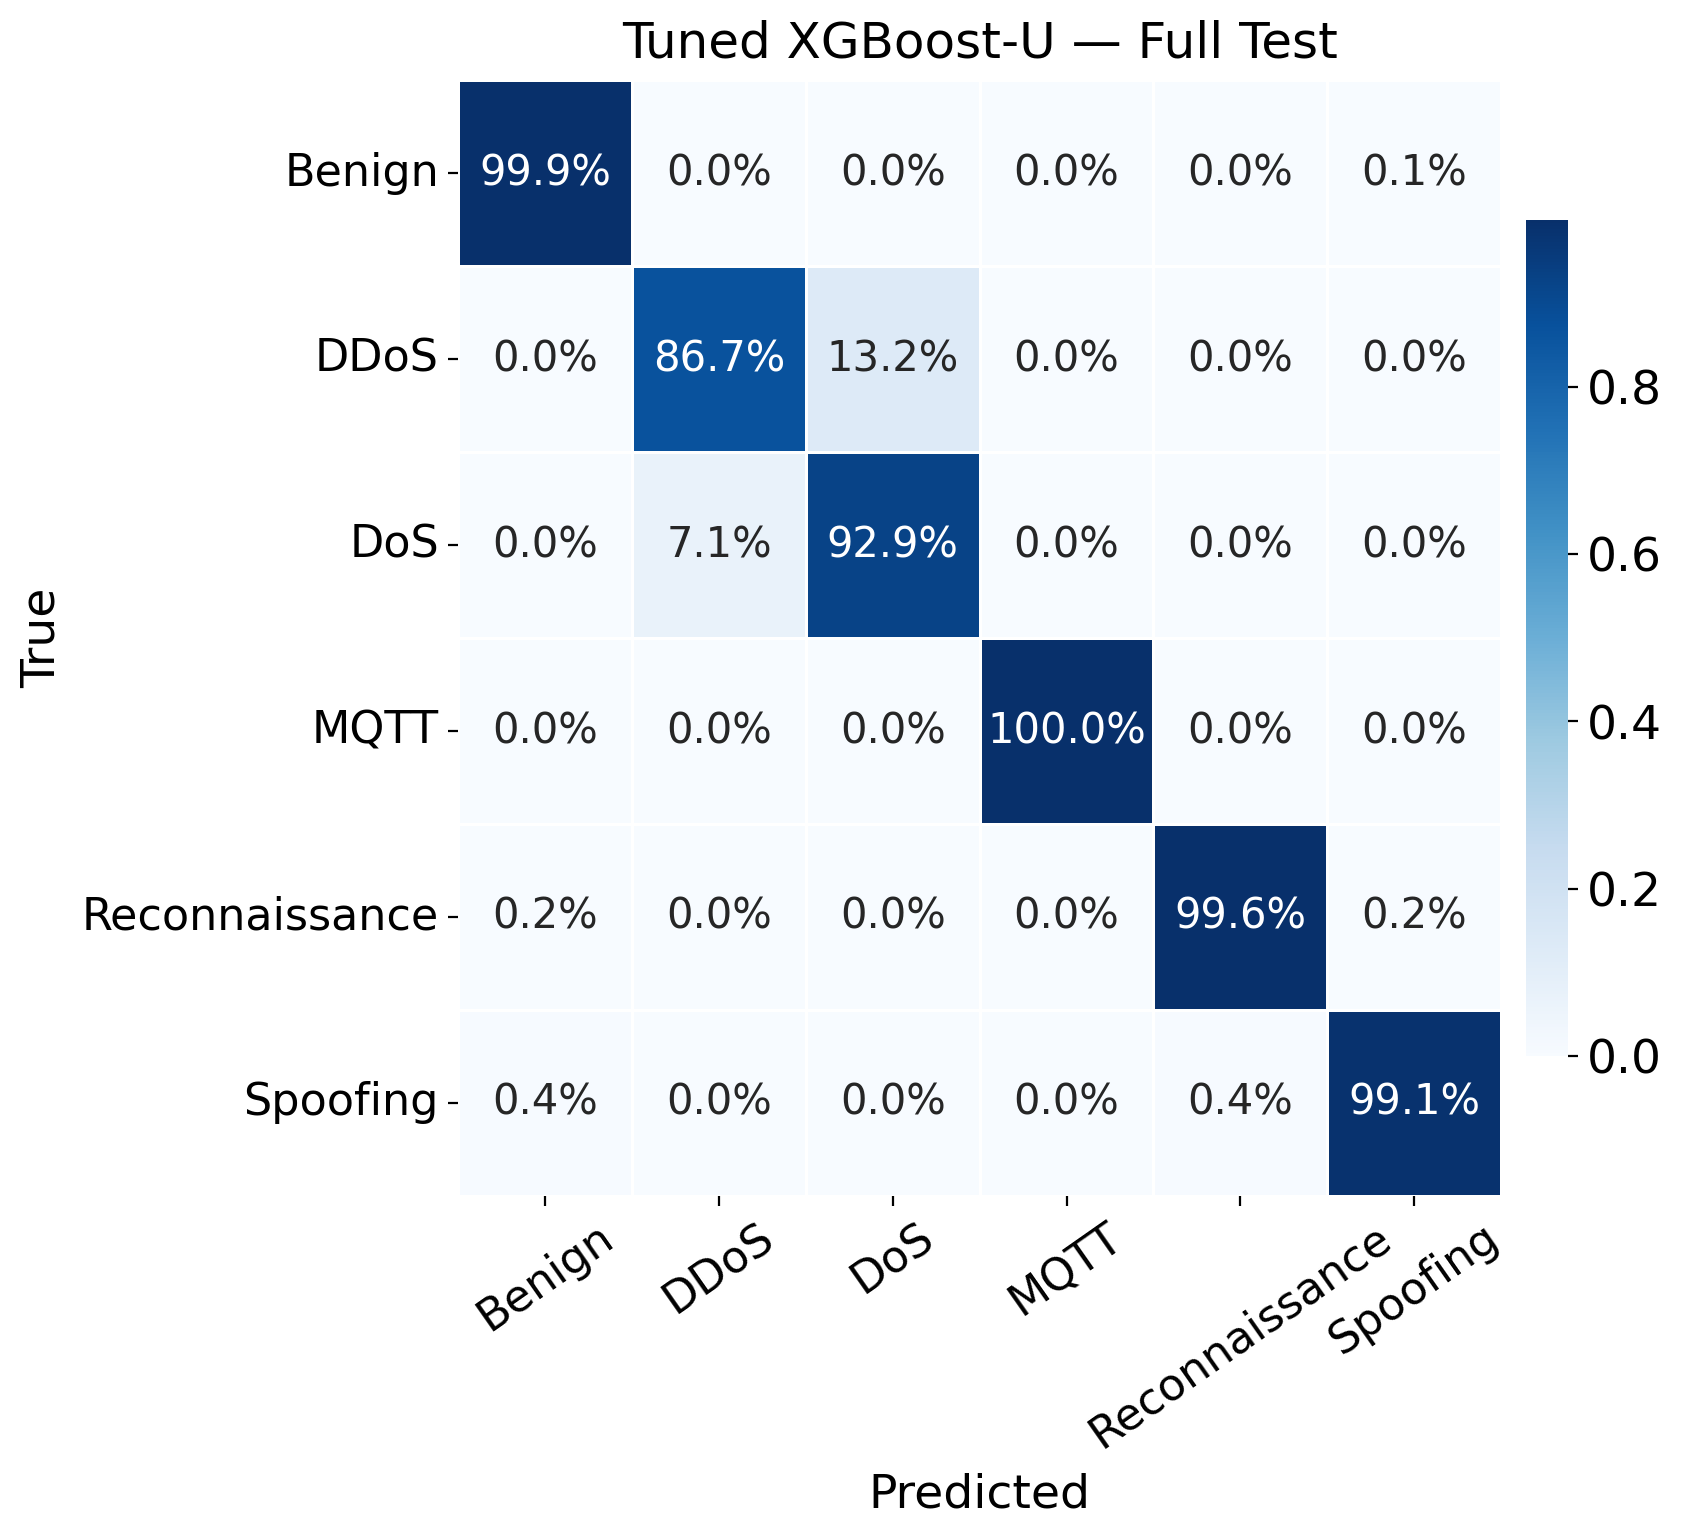
\includegraphics[width=0.81\textwidth]{cm_unified_xgb.png}
\caption{Normalized confusion matrix of the tuned XGBoost-U on the full mixed test set ($N=1{,}201{,}731$). Off-diagonal mass concentrates almost entirely on the DDoS$\leftrightarrow$DoS pair.}\label{fig:cm-unified}
\end{figure}

\begin{figure}[H]
\centering
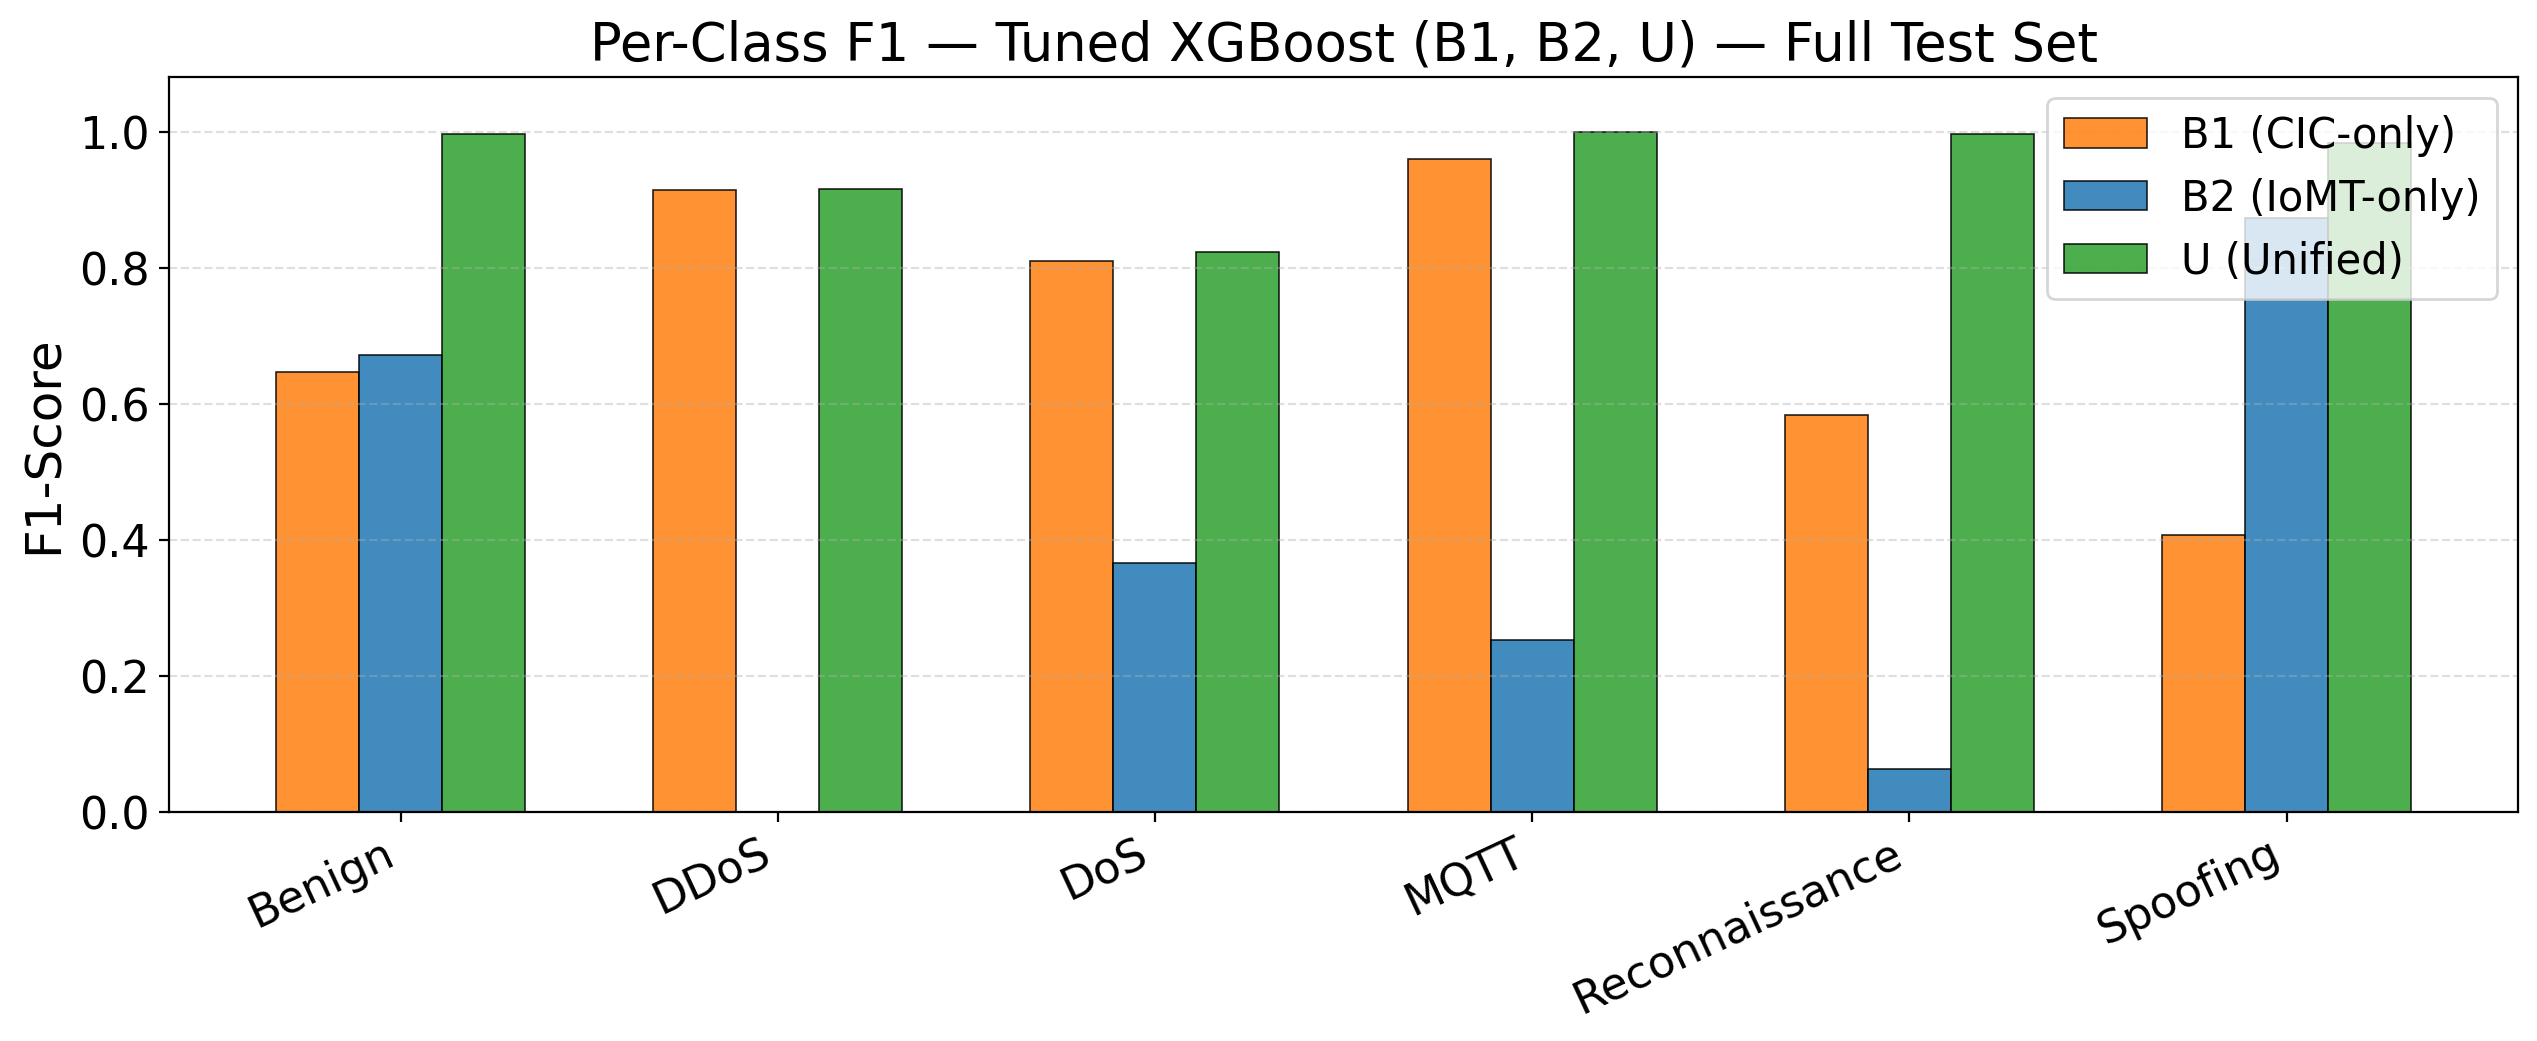
\includegraphics[width=0.90\textwidth]{per_class_f1.png}
\caption{Per-class F1 of the three tuned XGBoost regimes (B1, B2, U) on the full mixed test set. Single-source training (B1, B2) collapses on the off-source classes; the unified-trained model (U) recovers all six classes.}\label{fig:perclass}
\end{figure}

The dominant residual error is DDoS$\leftrightarrow$DoS confusion ($\approx$$13.3\%$ / $7.1\%$ cross-misclassification), accounting for $>99\%$ of errors---expected given similar flooding signatures in window statistics; capacity increases (DT$\to$RF$\to$XGB) narrow but do not remove this boundary.

\subsection{Cross-Domain Confusion Matrices}

Fig.~\ref{fig:xd-cm} shows the cross-domain confusion matrices for the tuned XGBoost models in B1$\to$IoMT and B2$\to$CIC. The patterns mirror Tables~\ref{tab:cross-domain}--\ref{tab:unified}: under B2$\to$CIC the absence of DDoS in training causes the model to misroute the dominant attack class to other categories, while B1$\to$IoMT preserves more diagonal mass but loses precision on the IoMT-specific MQTT and Reconnaissance traffic patterns.

\begin{figure}[H]
\centering
\begin{subfigure}[b]{0.50\textwidth}
  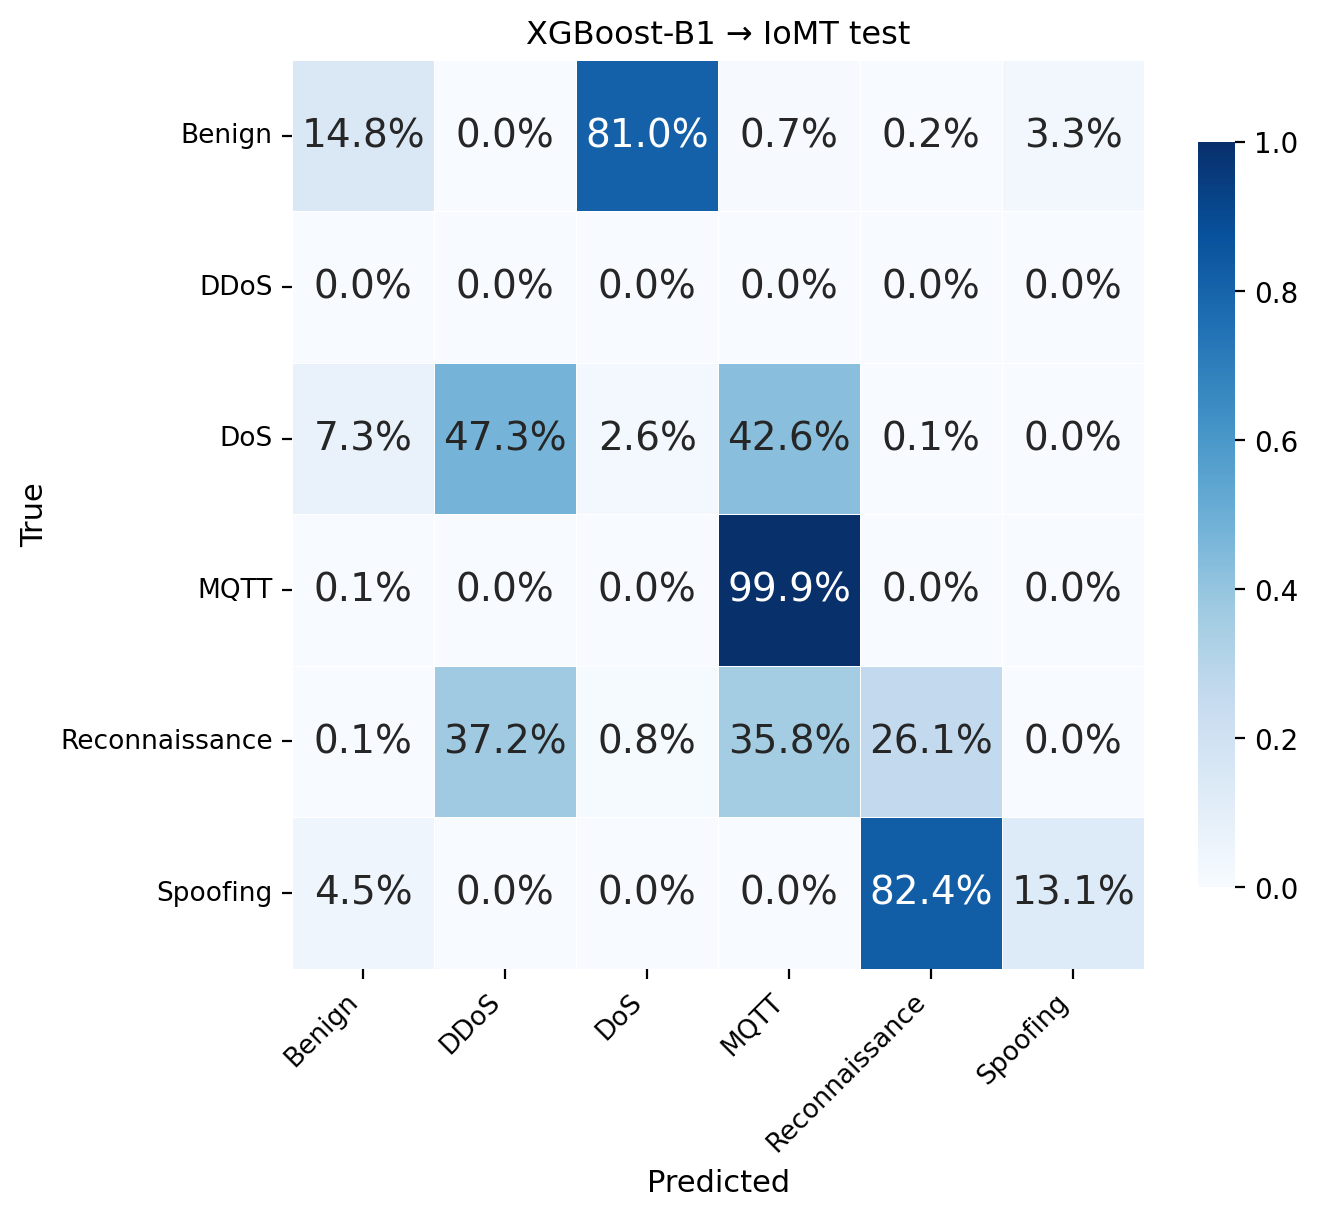
\includegraphics[width=\textwidth]{cm_b1_xd_iomt.png}
  \caption{XGBoost-B1 $\to$ IoMT test.}\label{fig:xd-b1}
\end{subfigure}\hfill
\begin{subfigure}[b]{0.50\textwidth}
  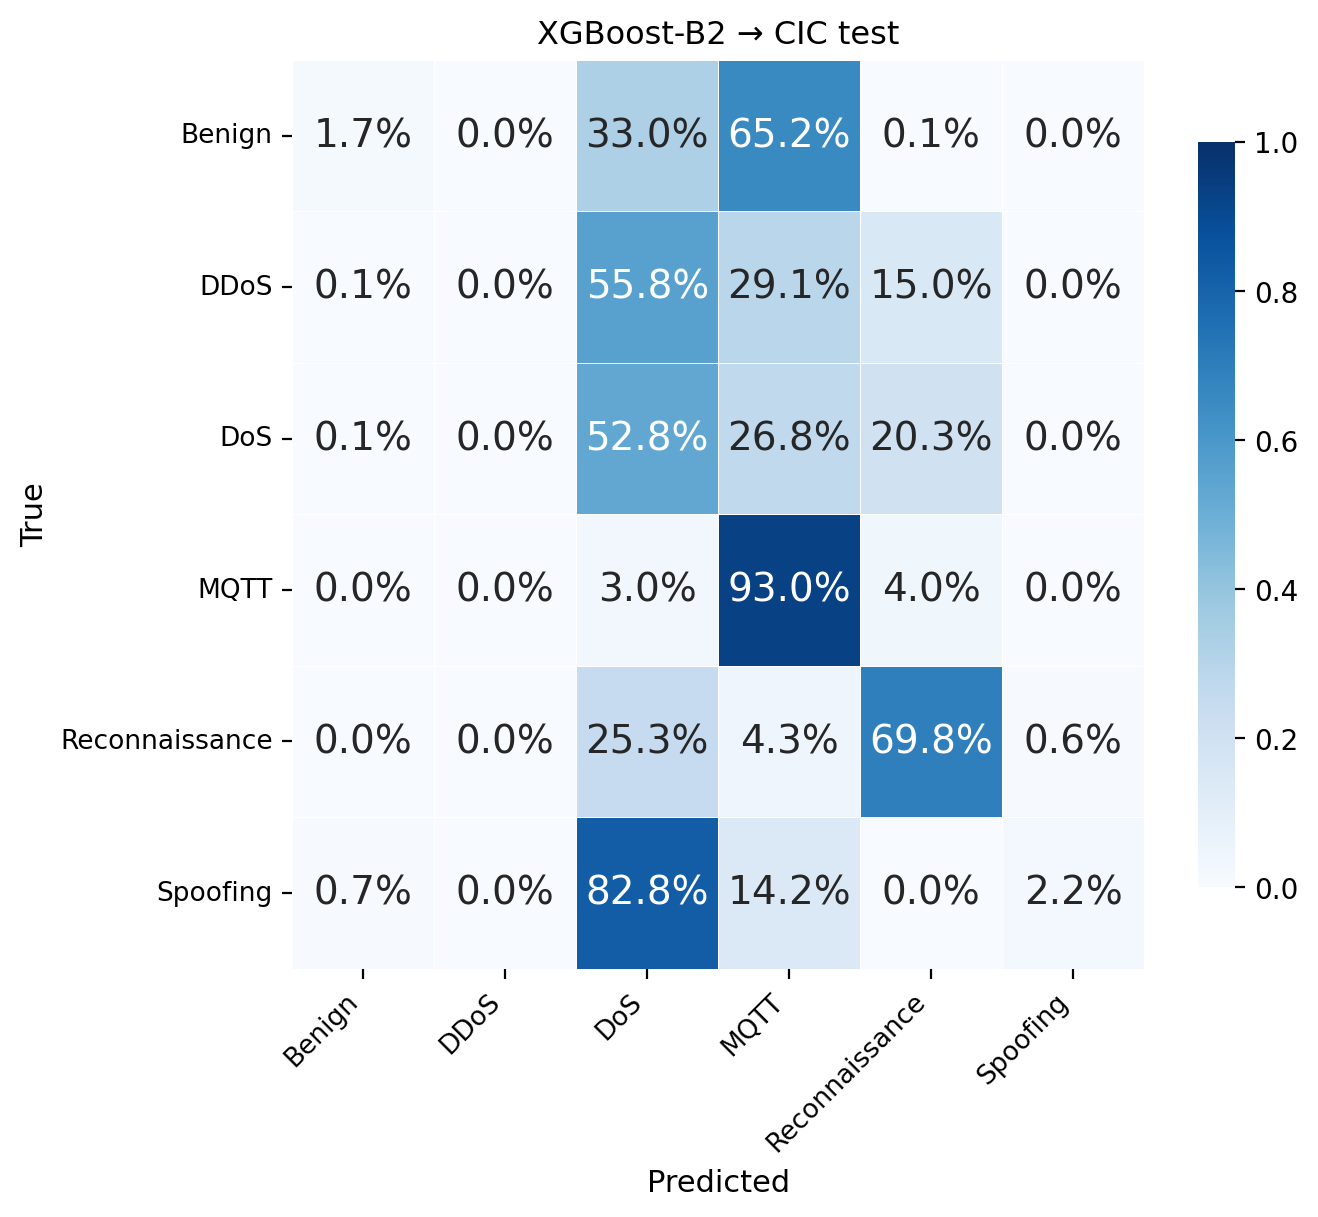
\includegraphics[width=\textwidth]{cm_b2_xd_cic.png}
  \caption{XGBoost-B2 $\to$ CIC test.}\label{fig:xd-b2}
\end{subfigure}
\caption{Cross-domain confusion matrices. B1 (CIC-only) loses precision on IoMT-specific classes; B2 (IoMT-only) misroutes the dominant CIC class (DDoS, absent from its training set).}\label{fig:xd-cm}
\end{figure}

\subsection{Statistical Significance: Pairwise McNemar Tests}
\label{subsec:mcnemar}

When two classifiers $A$ and $B$ are evaluated on the \emph{same} $N$ test examples, their per-example outcomes are not independent: every example contributes one prediction to each model. We therefore compare them with \textbf{McNemar's test}~\cite{mcnemar1947note}, the standard tool for paired binary outcomes and the recommended choice for comparing two classifiers on a single fixed test set~\cite{dietterich1998approximate}. For each example we only record whether $A$ and $B$ are individually correct or incorrect, and use the two off-diagonal cells of the resulting $2\!\times\!2$ contingency table: $b$ = examples where $A$ is right and $B$ is wrong, and $c$ = examples where $A$ is wrong and $B$ is right (the \emph{discordant} pairs). Examples where both are right or both are wrong carry no information about which model is better and are ignored. From $b$ and $c$ we compute the \textbf{Yates-corrected $\chi^{2}$ statistic} $\chi^{2}=(|b-c|-1)^{2}/(b+c)$ (the ``$-1$'' is a continuity correction); the associated \textbf{$p$-value} is the probability of observing such an imbalance between $b$ and $c$ if both models truly had identical error behaviour, so small $p$ means the difference is unlikely to be due to chance.

A naive two-proportion $z$-test on the two overall accuracies would treat the two error rates as if they came from independent samples, but here both rates come from the same examples, so that assumption is invalid. For multiclass outputs we apply the standard ``correct vs.\ incorrect'' per-example reduction~\cite{dietterich1998approximate}, which preserves the paired structure without requiring assumptions on full class-probability vectors. When more than two classifiers must be compared simultaneously, the natural extension is \textbf{Cochran's $Q$ test}~\cite{cochran1950q}; we keep pairwise McNemar tests so that each model pair has a directly interpretable result. Because $N>10^{6}$, even tiny differences become statistically significant, so $p$ alone is uninformative about practical importance. We therefore report the \textbf{Relative Error Reduction} $\mathrm{RER}(A\!\to\!B)=(e_A-e_B)/e_A\cdot 100\,\%$, where $e_A,e_B$ are the overall error rates of $A,B$: a positive RER means $B$ makes proportionally fewer errors than $A$. Table~\ref{tab:mcnemar} reports $b$, $c$, Yates $\chi^{2}$, $p$, and RER for all three pairs of unified-trained models on the full mixed test set ($N=1{,}201{,}731$).

\begin{table}[H]
\centering
\caption{Pairwise McNemar's test on the full mixed test set ($N = 1{,}201{,}731$). RER $> 0$ means the second model makes fewer errors.}\label{tab:mcnemar}
\small
\begin{tabular}{@{}lccrrr@{}}
\toprule
\textbf{Pair (A vs B)} & $b$ & $c$ & $\chi^{2}$ (Yates) & $p$-value & \textbf{RER (\%)} \\
\midrule
DT vs RF  & 6{,}919  & 6{,}372   & 22.43      & $2.2\times10^{-6}$ & $-0.41$ \\
DT vs XGB & 7{,}314  & 11{,}297  & 851.99     & $<10^{-15}$        & $+2.98$ \\
RF vs XGB & 4{,}246  & 8{,}776   & 1{,}575.17 & $<10^{-15}$        & $+3.38$ \\
\bottomrule
\end{tabular}
\end{table}

XGBoost is statistically and practically better than both DT and RF (RER $\approx 3\%$ corresponds to roughly $4{,}000$ fewer errors). The DT-vs-RF comparison is statistically significant but practically marginal: RF actually makes slightly more total errors than DT, although it has higher \macroF{} because it redistributes errors away from minority classes---the intended behaviour of class-balanced training.

\section{Real-World Evaluation: The HospNet26 Dataset}
\label{sec:results_2}

\subsection{Dataset and Protocol}

\textsc{HospNet26}~\cite{hospnet26,Domenech2026_cbms} is a publicly available reference dataset of anonymized network traffic features captured from the internal network of a Helios hospital (Germany) over one week of real clinical operation in August 2025. Unlike a laboratory IoMT testbed, it reflects the full hospital network---general IT, administrative, imaging, and IoT devices of all types, not exclusively IoMT. According to~\cite{Domenech2026_cbms}, the underlying captures contain raw traffic from $126$ distinct medical devices (e.g., imaging systems, blood analyzers, and sterilizers) across multiple manufacturers; device-level labels are unavailable in the released feature files, so medical-vs-IT proportions cannot be computed here. The four \emph{combined-feature} Parquet files (Friday, Weekend, Monday, Monday-to-Friday) provide $72$-column window-based + flow-level statistics per record. We extract the $58$ MIOTTA window-based features (a strict subset of the $72$ available columns) and concatenate the four files into a single evaluation set of $1{,}265{,}240$ windows. The remaining $14$ flow-level columns are discarded.

The dataset is \textbf{documented as containing only legitimate hospital traffic}: it was captured from a production clinical network during normal operation and released as a benign-traffic reference for IDS evaluation~\cite{hospnet26,Domenech2026_cbms}. Every window in our processed set has a known ground-truth class, namely \texttt{Benign}, and any non-Benign prediction by our models constitutes a false positive. To preserve a strict no-leakage protocol, we apply the \emph{same} \texttt{StandardScaler} fitted on the unified \emph{training} split (Section~\ref{sec:methodology}); no refitting on \textsc{HospNet26} is performed. The three tuned Unified models (DT-U, RF-U, XGB-U) are then run for inference without any retraining or adaptation.

\subsection{Evaluation Metric: Benign Prediction Rate}

Because all $1{,}265{,}240$ \textsc{HospNet26} windows share the same ground-truth class (\texttt{Benign}), the standard \macroF{}-over-six-classes is undefined. The appropriate metric is therefore the \textbf{Benign prediction rate} $r_{B}$, defined as the fraction of windows that the model classifies as \texttt{Benign}. In the present setting, $r_{B}$ is exactly the model's specificity (true-negative rate) on real clinical traffic; equivalently, $1\!-\!r_{B}$ is the false-positive rate, with the additional information of which attack class each false positive is mis-attributed to. A high $r_{B}$ indicates that the model correctly recognises live hospital traffic as legitimate; a low $r_{B}$ signals a distributional mismatch between the training-set Benign region and the operational environment.

\subsection{Results: A Substantial Laboratory-to-Clinic Gap}

Table~\ref{tab:hospnet} reports the predicted-class distribution for the three tuned Unified models on the $1.26 \times 10^{6}$ HospNet26 windows. The Benign prediction rate is $6.07\%$ for DT, $3.72\%$ for RF, and $9.96\%$ for XGBoost. The remaining $90\%\!-\!96\%$ of windows are classified as some form of attack, with $\sim$$51\%\!-\!72\%$ of all windows attributed to DoS.

\begin{table}[H]
\centering
\caption{HospNet26 prediction distribution: percentage of windows assigned to each class by the three tuned Unified models on $1{,}265{,}240$ real-hospital traffic windows. Because the dataset contains only legitimate clinical traffic, the last column (Benign rate $r_{B}$) is exactly the model's specificity on this deployment; all non-Benign columns are by construction false-positive rates.}\label{tab:hospnet}
\small
\begin{tabular}{@{}lrrrrrr|r@{}}
\toprule
\textbf{Model} & \textbf{Benign} & \textbf{DDoS} & \textbf{DoS} & \textbf{MQTT} & \textbf{Recon.} & \textbf{Spoofing} & \textbf{$r_{B}$} \\
\midrule
Decision Tree & 6.07\% &  7.80\% & 72.04\% & 0.22\% &  5.30\% &  8.57\% & \textbf{6.07\%} \\
Random Forest & 3.72\% &  0.60\% & 71.37\% & 0.06\% & 19.08\% &  5.17\% & \textbf{3.72\%} \\
XGBoost       & 9.96\% & 23.80\% & 51.14\% & 0.11\% &  4.28\% & 10.71\% & \textbf{9.96\%} \\
\bottomrule
\end{tabular}
\end{table}

A per-segment breakdown shows that \emph{Weekend} windows yield markedly lower Benign rates ($0.86\%\!-\!5.86\%$) than \emph{weekday} segments (Mon $5.02\%\!-\!11.57\%$, Fri $5.70\%\!-\!13.22\%$, Tue--Fri $5.18\%\!-\!12.12\%$), consistent with reduced administrative traffic on weekends moving the feature mix further from the laboratory training distribution.

\subsection{Does Multi-Source Integration Help on Real Clinical Traffic?}
\label{subsec:hospnet-regimes}

To isolate the effect of multi-source training on real-world specificity, we additionally apply the \emph{single-source} models from Section~\ref{sec:results_1} (B1: CIC-only, B2: IoMT-only) to \textsc{HospNet26}, with no other change to the inference pipeline. Table~\ref{tab:hospnet-regimes} reports the resulting Benign rate $r_{B}$ for all three regimes.

\begin{table}[H]
\centering
\caption{Benign prediction rate $r_{B}$ on \textsc{HospNet26} for the three training regimes ($N{=}1{,}265{,}240$ real-hospital windows). Higher is better; the column $\Delta_{U-\max(B_1,B_2)}$ shows how much regime U gains over the better of the two single-source models.}\label{tab:hospnet-regimes}
\small
\begin{tabular}{@{}lcccc@{}}
\toprule
\textbf{Model} & \textbf{B1 ($r_{B}$)} & \textbf{B2 ($r_{B}$)} & \textbf{U ($r_{B}$)} & \textbf{$\Delta_{U-\max(\text{B1},\text{B2})}$} \\
\midrule
Decision Tree & 9.16\%  & 0.00\%  & 6.07\%  & $-3.09$ pp \\
Random Forest & 4.61\%  & 5.46\%  & 3.72\%  & $-1.74$ pp \\
XGBoost       & 5.20\%  & 9.86\%  & \textbf{9.96\%} & $+0.10$ pp \\
\bottomrule
\end{tabular}
\end{table}

The pattern differs sharply from the laboratory test set, where regime U dominated both single-source baselines by $+20$ pp or more (Tables~\ref{tab:cross-domain}--\ref{tab:unified}). On real hospital traffic no regime systematically outperforms the others: all Benign rates fall within the same $0\%$--$10\%$ band regardless of training data composition, and the regime differences ($\leq 3$ pp) are negligible relative to the overall false-alarm burden ($90\%$--$96\%$). The laboratory-to-clinic gap is therefore not resolved by varying the laboratory training composition; it persists across all three regimes. This is consistent with the covariate-shift interpretation: all laboratory Benign samples---whether from CICIoMT2024, IoMT-TrafficData, or both---share the same fundamental mismatch with live clinical traffic, so no combination of these sources can move the Benign decision region toward the operational distribution. The result strengthens the case for the recalibration strategies of Section~\ref{sec:discussion}.

\subsection{Interpretation: Covariate Shift, Not Model Failure}

These results should not be read as a model failure. The same models achieve \macroF{} $\geq 0.948$ on the laboratory test set with virtually no benign misclassification. The sharp drop in specificity on \textsc{HospNet26} is an instance of \emph{covariate shift}~\cite{sommer2010outside}: the conditional distribution $p(x \mid y = \mathrm{Benign})$ in the training data differs systematically from the corresponding distribution in the deployment environment, while the per-class decision rules learned during training remain unchanged. Three concrete factors explain the gap:
\begin{enumerate}[nosep,leftmargin=*]
  \item \textbf{Laboratory benign traffic is not representative.} The Benign class in CICIoMT2024 and IoMT-TrafficData was generated in controlled testbed conditions (small device populations, synthetic baseline activity). Real hospital networks carry medical imaging streams (DICOM/PACS), electronic health record systems (HL7, FHIR), proprietary clinical device protocols, and large administrative back-office traffic, all with much higher volumes and different temporal patterns.
  \item \textbf{High-throughput clinical traffic resembles DoS.} Continuous PACS image streaming and bulk EMR synchronization produce burst-like packet statistics with high values of flow-rate and window-size features---the very features that the models have learned to associate with volumetric DoS attacks. This explains why DoS is the dominant false-positive class for all three models.
  \item \textbf{Weekday/weekend asymmetry.} The lower weekend Benign rates suggest that the laboratory training distribution is closer to ``office-hours'' clinical traffic than to weekend background activity, hinting at temporally non-stationary covariate shift that any deployment must confront.
\end{enumerate}

To the best of our knowledge, this is the first quantitative measurement of the laboratory-to-clinic gap for IoMT IDS. The implication is clear: strong laboratory benchmark performance is a necessary but not sufficient condition for safe operational deployment.

\section{Discussion}
\label{sec:discussion}

\subsection{What the Combined Evidence Says}

Two messages emerge from the combined evaluation. First, \textbf{multi-source dataset integration is decisive} for cross-source generalisation, raising full-mixed-test \macroF{} from $\leq 0.74$ (best single-source) to $\geq 0.948$ (any unified-trained model), with strong simultaneous performance on both constituent slices. Second, \textbf{laboratory generalisation does not imply operational generalisation}: even the best unified-trained model misclassifies $90\%\!-\!96\%$ of real clinical traffic, because its Benign decision region was learned from a non-representative testbed distribution. The second result \emph{qualifies} but does not invalidate the first: cross-source integration closes a real gap among laboratory benchmarks, but not the orthogonal lab-to-clinic gap.

\subsection{Recalibration Strategies}

The HospNet26 finding suggests two concrete, low-cost recalibration strategies that practitioners can deploy without renouncing the benefits of multi-source integration. \textbf{Few-shot Benign fine-tuning} adds a small, supervised collection of confirmed-benign hospital traffic ($10{,}000$--$50{,}000$ windows) to the training set and retrains the model: this shifts the Benign decision boundary toward real clinical statistics while preserving attack-detection capability; collection effort is modest since any live capture yields $>\!10^{6}$ windows per week. \textbf{Threshold-based post-hoc calibration} instead keeps the existing model and recalibrates its probability outputs (e.g.\ XGBoost \texttt{predict\_proba}) on a held-out set of known-benign hospital windows; a class-specific decision threshold is then optimized to trade off false-positive rate against detection sensitivity (e.g.\ targeting $\leq 1\%$ false alarms). Both strategies require only \emph{benign} traffic, abundant in any live network, and avoid the ethical and practical issues of labelled attack collection in a real hospital.

\subsection{Threats to Validity}

Four threats to validity remain: (i) we evaluate \emph{tree-based models only}; packet-level deep models~\cite{holland2021nprint} may interact differently with covariate shift and are prioritized in future work; (ii) all experiments use a fixed MIOTTA-NPT window size ($W{=}100$) and a fixed $58$-feature window representation, so sensitivity to alternative window sizes, feature-group ablations, and per-packet binary mode remains unexplored; (iii) the integration uses \emph{two} sources, so adding a third (e.g.\ CICIoT2023~\cite{neto2023ciciot2023}) may expose attack-class coverage gaps not visible here; (iv) the recalibration strategies are described but not yet empirically validated.

\section{Conclusion and Future Work}
\label{sec:conclusion}

This paper addressed two interconnected limitations of current ML-based IDS for IoMT environments: dataset isolation with feature heterogeneity, and the absence of evaluation against real clinical traffic. We proposed a PCAP-level integration methodology built on the MIOTTA-NPT preprocessing tool, a three-level label harmonization scheme, source-attribution metadata, and stratified cross-domain splitting. The resulting unified dataset of $8 \times 10^{6}$ records enables three tree-based classifiers to reach \macroF{} up to $0.952$ on the full mixed test set and $\geq 0.926$ on each constituent source slice, dramatically outperforming all single-source baselines (factor $\sim 50\times$ vs.\ model complexity). Beyond laboratory results, we presented the first evaluation of an IoMT IDS on \textsc{HospNet26} and showed that Benign rates on $1.26\!\times\!10^{6}$ live clinical windows ($3.7\%\!-\!10.0\%$) reveal a substantial laboratory-to-clinic covariate shift, motivating few-shot Benign fine-tuning and post-hoc threshold calibration as practical strategies for closing the gap. 

Future work could focus on five natural directions:
(i)~empirical validation of the recalibration strategies, quantifying how many supervised benign hospital windows are needed to reach $r_{B} \geq 0.90$;
(ii)~extension to a third source (e.g.\ CICIoT2023~\cite{neto2023ciciot2023}) via the same MIOTTA-NPT pipeline;
(iii)~packet-level deep architectures~\cite{holland2021nprint} and sensitivity analysis over window size (e.g.\ $W \in \{50,100,200\}$), feature-group ablation, and MIOTTA-NPT per-packet binary mode;
(iv)~feature engineering targeted at the DDoS--DoS boundary (e.g.\ source-address diversity, flow-volume asymmetry);
(v)~an operational deployment study tracking concept drift and alert fatigue with recalibrated models.

\subsubsection*{Acknowledgments.}
This work was supported by the AGAUR-FI Joan Oró program (2024 FI-1 00643) and the CARISMATICA Chair of Cybersecurity. The funding is provided by the Secretariat of Universities and Research (Generalitat of Catalonia), with additional support from the EU and INCIBE.

\subsubsection*{Disclosure of Interests.}
The authors declare no competing interests relevant to the content of this article.

{\small
\vspace{-2mm}
\let\oldthebibliography\thebibliography
\renewcommand{\thebibliography}[1]{\oldthebibliography{#1}\setlength{\itemsep}{-0.5pt plus 0.1ex}\setlength{\parskip}{0pt}}
\bibliographystyle{splncs04}
\bibliography{references}
}

\end{document}
